%%%%%%%%%%%%%%%%%%%%%%%%%%%%%%%%%%%%%%%%%
% University/School Laboratory Report
% LaTeX Template
% Version 3.0 (4/2/13)
%
% This template has been downloaded from:
% http://www.LaTeXTemplates.com
%
% Original author:
% Linux and Unix Users Group at Virginia Tech Wiki 
% (https://vtluug.org/wiki/Example_LaTeX_chem_lab_report)
%
% License:
% CC BY-NC-SA 3.0 (http://creativecommons.org/licenses/by-nc-sa/3.0/)
%
%%%%%%%%%%%%%%%%%%%%%%%%%%%%%%%%%%%%%%%%%

%----------------------------------------------------------------------------------------
%	PACKAGES AND DOCUMENT CONFIGURATIONS
%----------------------------------------------------------------------------------------

\documentclass{article}

\usepackage[version=3]{mhchem} % Package for chemical equation typesetting
\usepackage{siunitx} % Provides the \SI{}{} command for typesetting SI units

\usepackage{graphicx}
\usepackage{caption}
\usepackage{subcaption}

\usepackage{float}

\usepackage[T1]{fontenc} % allow small bold caps

\usepackage{listings}
\usepackage{color}

\definecolor{dkgreen}{rgb}{0,0.6,0}
\definecolor{gray}{rgb}{0.5,0.5,0.5}
\definecolor{mauve}{rgb}{0.58,0,0.82}

\lstset{frame=tb,
  language=Python,
  aboveskip=2mm,
  belowskip=2mm,
  showstringspaces=false,
  columns=flexible,
  basicstyle={\small\ttfamily},
  numbers=none,
  numberstyle=\tiny\color{gray},
  keywordstyle=\color{blue},
  commentstyle=\color{dkgreen},
  stringstyle=\color{mauve},
  breaklines=true,
  breakatwhitespace=true
  tabsize=2
}

\setlength\parindent{0pt} % Removes all indentation from paragraphs

\renewcommand{\labelenumi}{\alph{enumi}.} % Make numbering in the enumerate environment by letter rather than number (e.g. section 6)

\usepackage[margin=1in]{geometry}

\usepackage{amssymb}

%\usepackage{times} % Uncomment to use the Times New Roman font

%----------------------------------------------------------------------------------------
%	Title
%----------------------------------------------------------------------------------------

\begin{document}
\pagenumbering{gobble}

\title{6.036: Machine Learning}
\author{
  Ryan Lacey <rlacey@mit.edu>\\
}
        
\maketitle
        

\begin{enumerate}
\item[4.]
	Small values of $l$ ($\le$ 50 components) performed poorly on reconstruction of the images. For $l \ge 500$ most of the detail of the original images is restored and the blur effect is marginal.\\
	
	\begin{figure}[!htb]
	\minipage{0.30\textwidth}
	  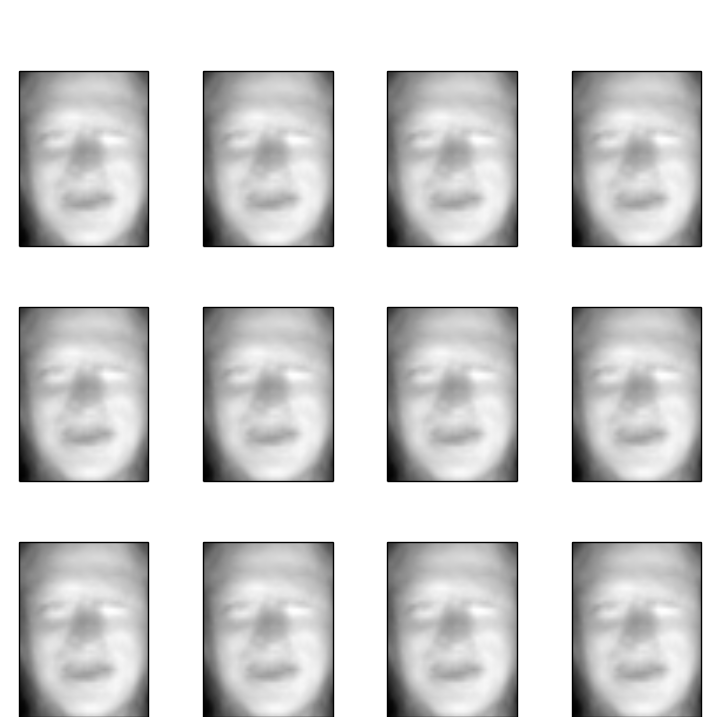
\includegraphics[width=\linewidth]{../images/reconstructed1.png}
	  \caption{1 component}
	\endminipage\hfill
	\minipage{0.30\textwidth}
	  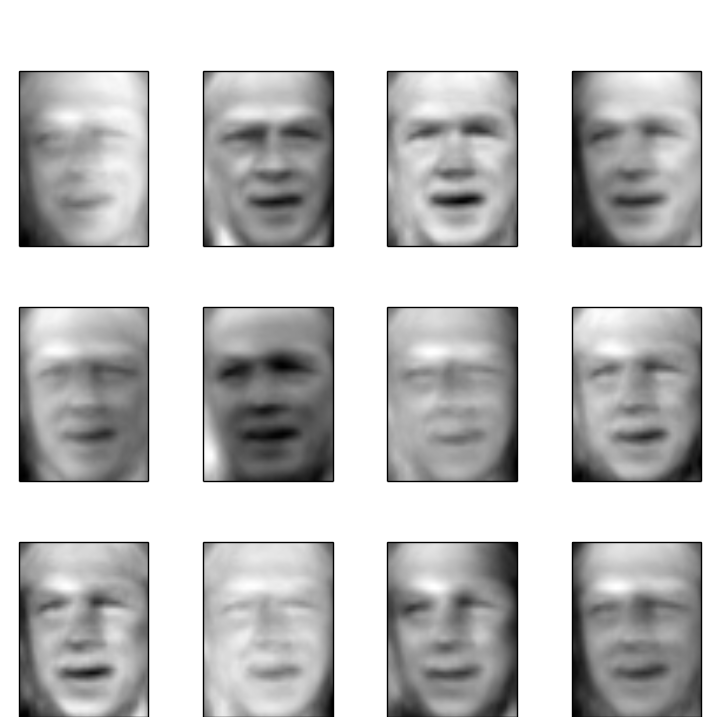
\includegraphics[width=\linewidth]{../images/reconstructed10.png}
	  \caption{10 components}
	\endminipage\hfill
	\minipage{0.30\textwidth}
	  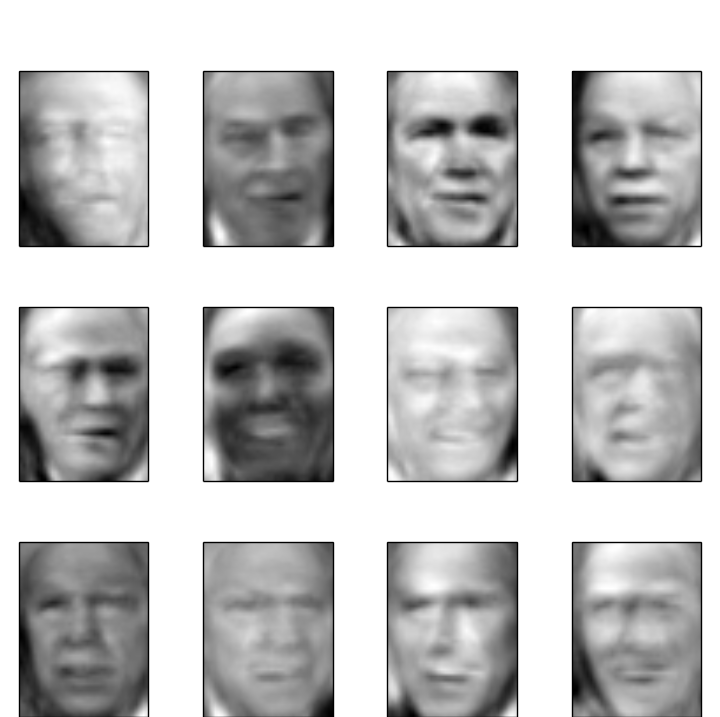
\includegraphics[width=\linewidth]{../images/reconstructed50.png}
	  \caption{50 components}
	\endminipage\hfill
	\end{figure}
	\begin{figure}[!htb]
	\minipage{0.30\textwidth}
	  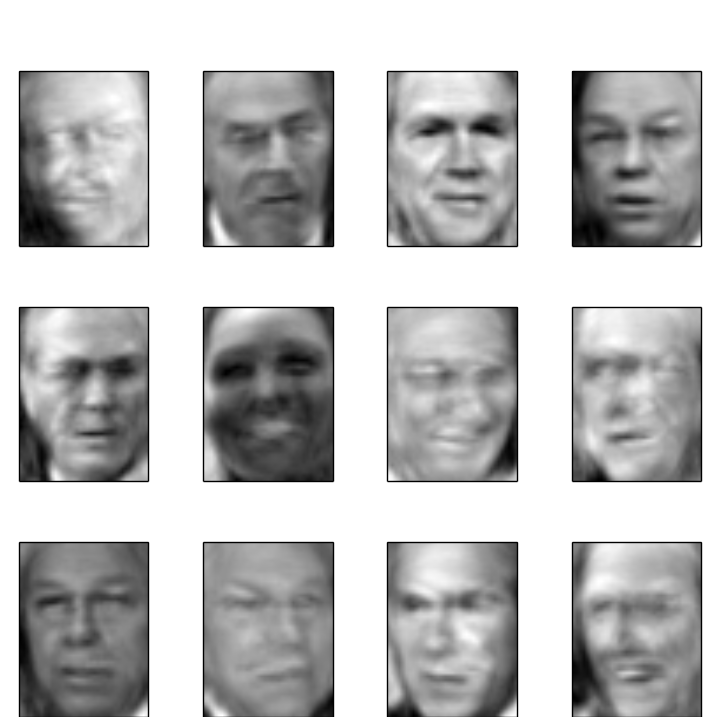
\includegraphics[width=\linewidth]{../images/reconstructed100.png}
	  \caption{100 components}
	\endminipage\hfill
	\minipage{0.30\textwidth}
	  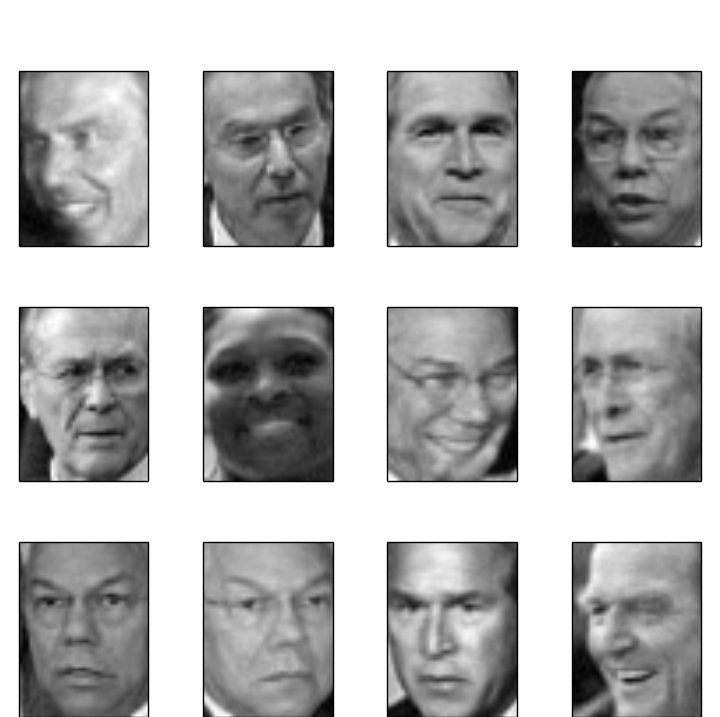
\includegraphics[width=\linewidth]{../images/reconstructed500.png}
	  \caption{500 components}
	\endminipage\hfill
	\minipage{0.30\textwidth}
	  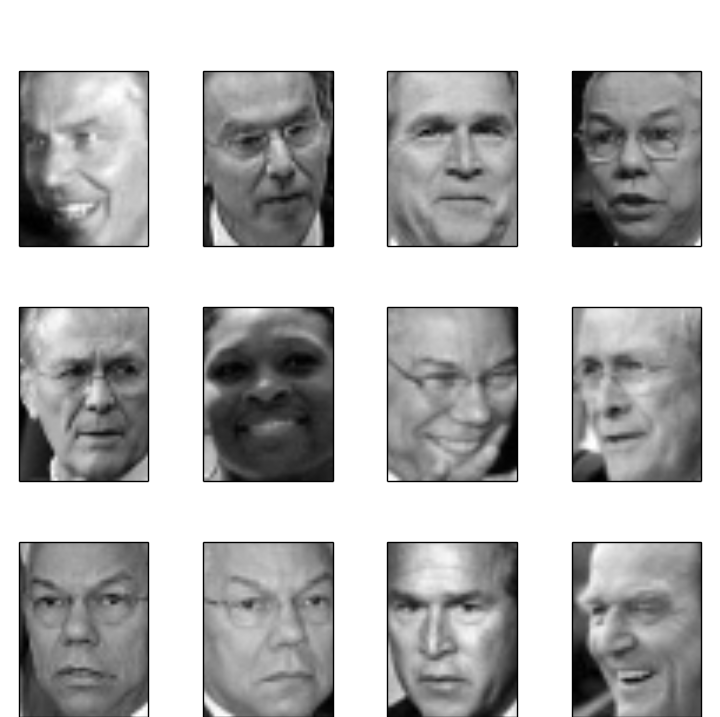
\includegraphics[width=\linewidth]{../images/reconstructed1288.png}
	  \caption{1288 components}
	\endminipage\hfill
	\end{figure}

\bigskip 

\begin{lstlisting}   
# l integer value specifying quantity of components
def reconstruct(l):
    E, mu = PCA(X)
    Z = X.dot(E[:, 0:l])
    print Z.shape
    print E.T[0:l].shape
    reconstructed = Z.dot(E.T[0:l])
    plotGallery([reconstructed[i] for i in range(12)])
\end{lstlisting}


\newpage

\item[5.]
	The error rates for the training and test data remain relatively constant until the value of $C$ become sufficiently large. It makes sense that the error decreases with an increase of $C$ because larger values of $C$ permit fewer violations, forcing the margins of the SVM to become tighter. Note that the curves remain nearly the same in value and shape across all values of $C$. Therefore it is best for this data to choose a large $C$ in order to minimize the number of misclassifications, because we can expect that the separator will still generalize well. \\
	
	\begin{figure}[!htb]
	\begin{center}
	\minipage{0.65\textwidth}
	  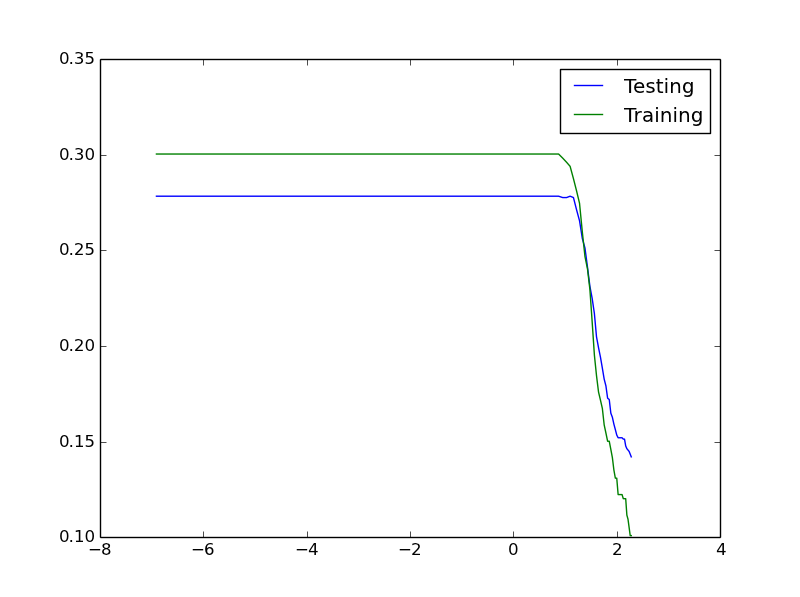
\includegraphics[width=\linewidth]{../images/ClassificationErrorC.png}
	  \caption{Training and test error as a function of $\log(C)$}
	\endminipage\hfill
	\end{center}
	\end{figure}

\bigskip 

\begin{lstlisting}   
def dataRangeC():
    Cs = np.arange(0.001,10,0.2)
    testingError = []
    trainingError = []
    E, mu = PCA(X, True)
    Z = X.dot(E[:, 0:100])
    newY = [+1 if yi == 4 else -1 for yi in y]
    (X1, X2, y1, y2) = sklearn.cross_validation.train_test_split(Z, newY, test_size=.75)
    for C in Cs:
        clf = SVC(kernel='linear', C=C)
        clf.fit(X1, y1)
        score = clf.score(X2, y2)
        testingError.append(1-score)
        score = clf.score(X1, y1)
        trainingError.append(1-score)
    return Cs, testingError, trainingError
\end{lstlisting}

\newpage

\item[6.]
	In general the training and test error decreases as $l$ increases. While the decrease in error for testing data plateaus, however, the training data continues to show improvement. Since we care about the performance on the generalized data set, the point at which the plateau of test error begins would be the optimal choice of $l$. This is because it would minimize the training efforts, as there would be less data to compute on with the smaller number of components, and the performance at that point is about as good as it can get for any value $l$ selected. Note that the sporadic increase/decrease nature of the error with increasing $l$ comes from the fact that each new value of $l$ required retraining on a new test set to incorporate the additional components.\\
	
	\begin{figure}[!htb]
	\begin{center}
	\minipage{0.65\textwidth}
	  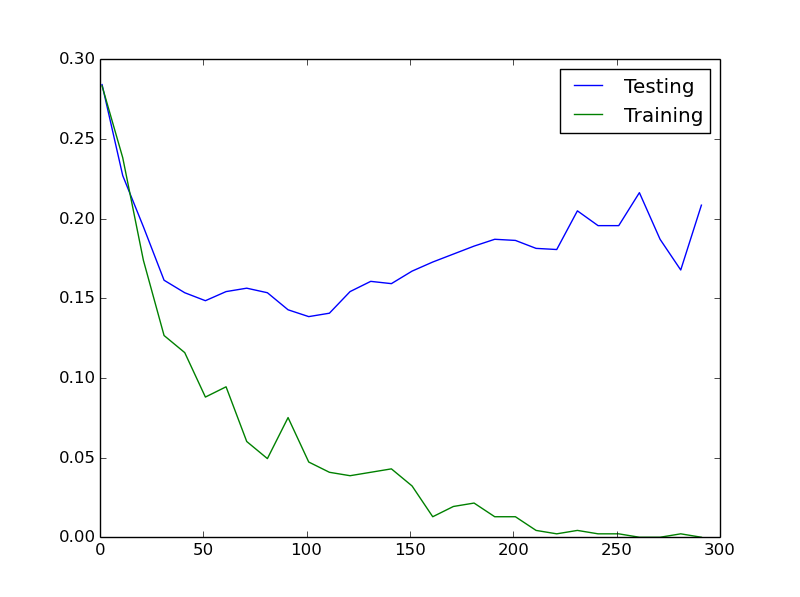
\includegraphics[width=\linewidth]{../images/ClassificationErrorComponents.png}
	  \caption{Training and test error as a function of $l$ (components)}
	\endminipage\hfill
	\end{center}
	\end{figure}

\bigskip 

\begin{lstlisting}   
def dataRangeComponent():
    Ls = np.arange(1,300,10)
    testingError = []
    trainingError = []
    E, mu = PCA(X, True)
    newY = [+1 if yi == 4 else -1 for yi in y]
    for L in Ls:
        Z = X.dot(E[:, 0:L])
        (X1, X2, y1, y2) = sklearn.cross_validation.train_test_split(Z, newY, test_size=.75)
        clf = SVC(kernel='linear', C=100)
        clf.fit(X1, y1)
        score = clf.score(X2, y2)
        testingError.append(1-score)
        score = clf.score(X1, y1)
        trainingError.append(1-score)
    return Ls, testingError, trainingError
\end{lstlisting}

\newpage

\item[7.]
	Example progression of example k\_means algorithm to sample data. Demonstrates how centroids move in a well clustered system. Correct classification is achieved even if the starting location of the centroids is not near their respective clusters and the initial data points are not labeled as they would be in the final state.\\
	
	\begin{figure}[!htb]
	\begin{center}
	\minipage{0.6\textwidth}
	  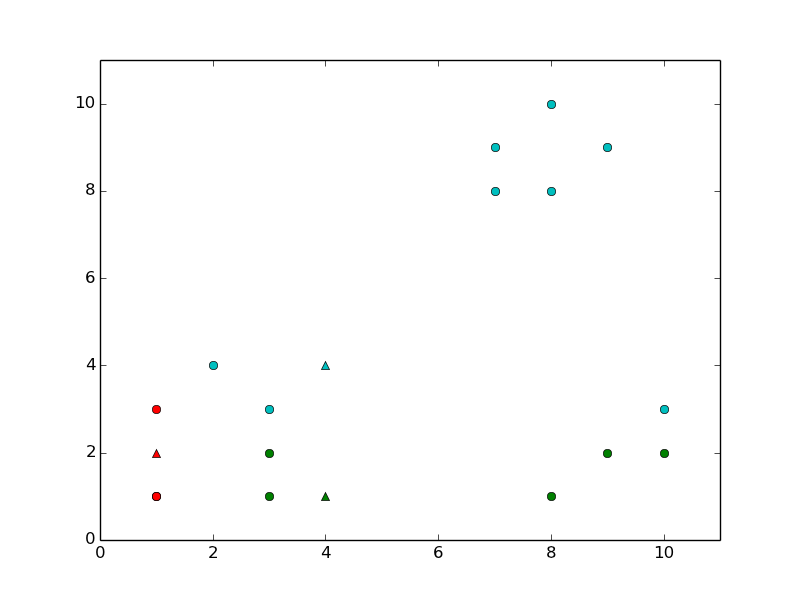
\includegraphics[width=\linewidth]{../images/Cluster1.png}
	  \caption{Initial system state with data points represented with circles and centoids represented with triangles. The color of each points represents which cluster it is a part of with the representatives of the clusters being the centroids.}
	\endminipage\hfill
	\end{center}
	\end{figure}
	\begin{figure}[!htb]--
	\minipage{0.48\textwidth}
	  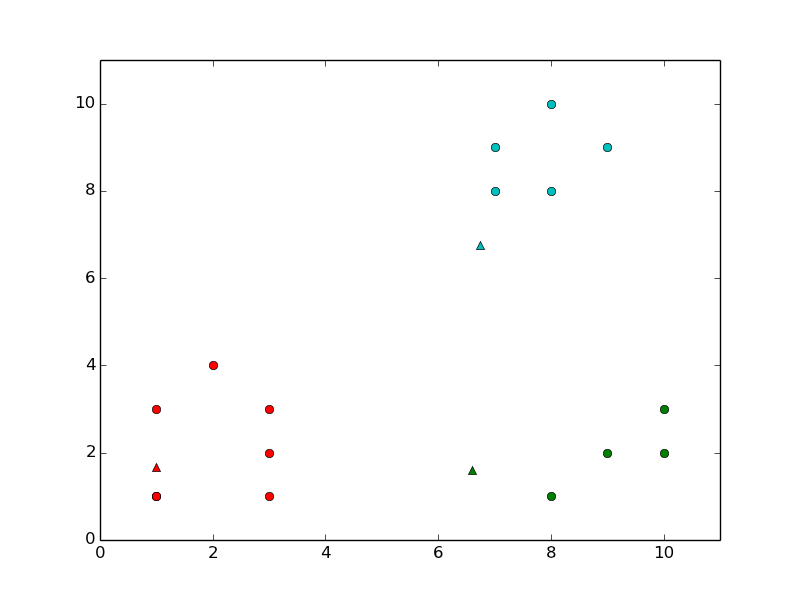
\includegraphics[width=\linewidth]{../images/Cluster2.png}
	  \caption{First update state with all points attributed to correct centroid}
	\endminipage\hfill
	\minipage{0.48\textwidth}
	  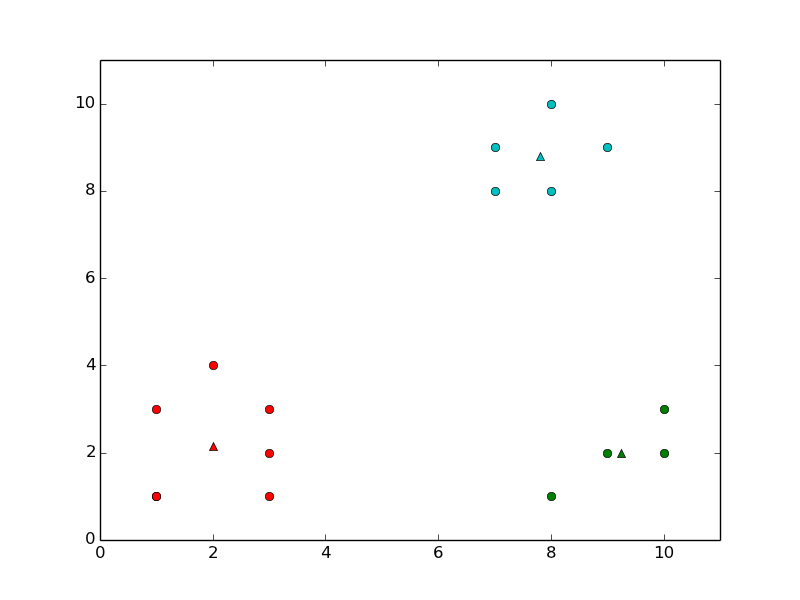
\includegraphics[width=\linewidth]{../images/Cluster3.png}
	  \caption{Final state with centroids at center of respective clusters}
	\endminipage\hfill
	\end{figure}

\newpage 

\begin{lstlisting}   
def ml_k_means(X, init):
    number_of_points = len(X)
    number_of_clusters = len(init)
    centroids = init.astype(float)
    clusterAssignments = np.array([0]*number_of_points)
    totalCost = float('inf')
    costs = np.array([float('inf')]*number_of_points)
    # Set initial closest representitive for every point
    for i in range(number_of_points):
        for j in range(number_of_clusters):
            pointCost = np.linalg.norm(X[i]-centroids[j])
            if pointCost <  costs[i]:
                clusterAssignments[i] = j
                costs[i] = pointCost 
    # Move representitive to center of cluster and reassign points
    while True:                            
        for j in range(number_of_clusters):
            points_in_cluster = np.array([x for i, x in enumerate(X) if clusterAssignments[i]==j])
            cluster_sum = np.sum(points_in_cluster, axis=0)
            centroids[j] = cluster_sum / float(len(points_in_cluster))
        costs = np.array([float('inf')]*number_of_points)
        for i in range(number_of_points):
            for j in range(number_of_clusters):
                pointCost = np.linalg.norm(X[i]-centroids[j])
                if pointCost <  costs[i]:
                    clusterAssignments[i] = j
                    costs[i] = pointCost                 
        newCost = np.sum(costs)
        if newCost == totalCost:
            break
        totalCost = newCost       
    return centroids, clusterAssignments
\end{lstlisting}

\newpage

\item[8.]
	The cheat initializer performed as well as the best of the random initializations and on average well outperforms the randomly positioned starting medoids. This should be expected because it used class information in selecting the start metoids.\\
	
	Cheat initialization scores: 0.8125\\
	Random initialization scores: 0.7125, 0.775, 0.7875, 0.775, 0.8125, 0.7125, 0.5, 0.5, 0.7875, 0.7125\\
	
	Average random initialization score: 0.71\\

\newpage

\begin{lstlisting}   
def ml_k_medoids(X, init):
    number_of_points = len(X)
    number_of_clusters = len(init)
    medoids = init.astype(float)
    clusterAssignments = np.array([0]*number_of_points)
    totalCost = float('inf')
    while True:         
        # Update cluster assignments
        costs = np.array([float('inf')]*number_of_points)
        for i in range(number_of_points):
            for j in range(number_of_clusters):
                pointCost = np.linalg.norm(X[i]-medoids[j])
                if pointCost <  costs[i]:
                    clusterAssignments[i] = j
                    costs[i] = pointCost                                   
        newCost = np.sum(costs)
        if newCost == totalCost:
            break
        totalCost = newCost                                          
        # Choose new exemplars    
        costs = np.array([float('inf')]*number_of_clusters)                      
        for j in range(number_of_clusters):
            points_in_cluster = np.array([x for i, x in enumerate(X) if clusterAssignments[i]==j])
            for proposed in points_in_cluster:
                cost = 0
                for x in points_in_cluster:
                    cost += np.linalg.norm(proposed-x)
                if cost < costs[j]:
                    medoids[j] = proposed
                    costs[j] = cost     
    return medoids, clusterAssignments
    
def cheatScoring():
    X1, y1 = limitPics(X, y, [4, 13], 40)
    init, indecies = cheatInit(X1, y1, 2)
    medoids, clusters = ml_k_medoids(X1, init)
    return scoreMedoids((medoids, indecies, clusters), y1)
    
def randomScoring():
    X1, y1 = limitPics(X, y, [4, 13], 40)
    r1 = int(random.random()*X1.shape[0])
    r2 = int(random.random()*X1.shape[0])
    init = np.array([X1[r1], X1[r2]])
    medoids, clusters = ml_k_medoids(X1, init)
    indecies = [None, None]
    for i, x in enumerate(X1):
        if np.array_equal(x, medoids[0]): indecies[0] = i
        if np.array_equal(x, medoids[1]): indecies[1] = i
    return scoreMedoids((medoids, indecies, clusters), y1)
\end{lstlisting}

\newpage

\item[9.]
	The metoid scoring function output generally increases when more components are incorporated. When about 25\% of the components are used (10 out of 40 for this dataset) the gains become marginal and the scores began to plateau. The difference in scores for different $l$ values is greatest when $l$ is small. This makes sense because, for example, having two components vs six components is a threefold difference in information. 

\bigskip

	\begin{figure}[!htb]
	\begin{center}
	\minipage{0.6\textwidth}
	  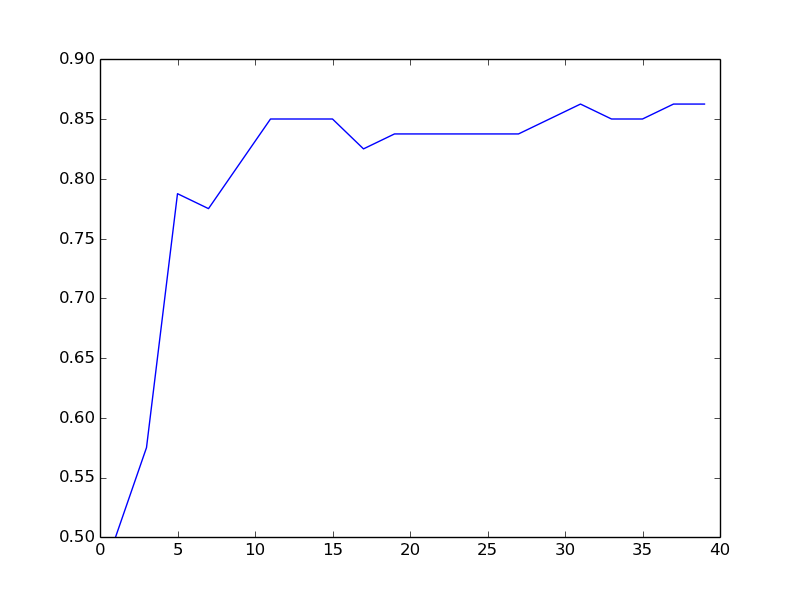
\includegraphics[width=\linewidth]{../images/PCAscoring.png}
	  \caption{Score as a function of the number of components}
	\endminipage\hfill
	\end{center}
	\end{figure}

\bigskip

\begin{lstlisting}   
def pcaScoring():
    E, mu = PCA(X)
    Ls = np.arange(1,40,2)
    scores = []
    for L in Ls:
        Z = X.dot(E[:, 0:L])
        X1, y1 = limitPics(Z, y, [4, 13], 40)
        init, indecies = cheatInit(X1, y1, 2)
        medoids, clusters = ml_k_medoids(X1, init)
        scores.append(scoreMedoids((medoids, indecies, clusters), y1))
    plt.figure("PCA Scoring") 
    plt.plot(Ls, scores)
    return scores
\end{lstlisting}

\newpage

\item[10.]
	The hardest pictures to discriminate were 4 and 5, because they had the lowest metroid score (score = 0.5). Pictures 6 and 16 on the other hand discriminated well (score = 1.0). These combinations were found by trying all combinations of the 19 classes. The score of the hardest suggests that our ability to correctly cluster is as good as flipping a coin and randomly choosing a clluster for the data point. The score of the easy pictures, on the other hand, suggests that we will always correctly classify the data points. 

\bigskip

\begin{lstlisting}   
def pairsScoring():
    hardestScore = 1
    easiestScore = 0
    hardest = [None, None]
    easiest = [None, None]
    for i in range(19):
        for j in range(19): 
            if i != j:       
                X1, y1 = limitPics(X, y, [i, j], 40)
                init, indecies = cheatInit(X1, y1, 2)
                medoids, clusters = ml_k_medoids(X1, init)
                score = scoreMedoids((medoids, indecies, clusters), y1)
                if score < hardestScore:
                    hardestScore = score
                    hardest = [i, j]
                if score > easiestScore:
                    easiestScore = score
                    easiest = [i, j]                
    return hardest, easiest
\end{lstlisting}

\end{enumerate}

\end{document}